\section{Просодическая обработка синтезированных фраз}

\subsection{Задание 3.3.6*. Контуры мелодики, ритмики и энергетики}

Для придания синтезированным фразам интонационной насыщенности заданы три
просодических контура:
\begin{itemize}
	\item $F_0(t)$ --- мелодический: сдвиг тона каждого слога в полутонах;
	\item $A(t)$ --- энергетический: добавка к уровню каждого слога, дБ;
	\item $T(t)$ --- ритмический: коэффициент длительности каждого слога.
\end{itemize}
Значения подобраны по измеренным контурам эталонных фраз: в вопросе тон
повышается к концу, в утверждении и перечислении --- понижается, ударные
слоги удлиняются и усиливаются. Сдвиг тона выполнялся с \emph{сохранением
формант}: оболочка спектра (тембр гласного) не изменялась, а смещались
только гармоники, поэтому голос не <<менялся>>, а лишь повышался или
понижался. Заданные контуры приведены в таблице~\ref{tab:prosody}, их
применение и результат --- на рисунке~\ref{fig:prosody}.

\begin{table}[H]
	\centering
	\footnotesize
	\caption{Просодические контуры синтезируемых фраз}
	\label{tab:prosody}
	\begin{tabular}{|l|l|c|c|c|c|c|}
		\hline
		Фраза & Слог & $\Delta F_0$, пт & $\Delta A$, дБ & $T$ &
		$F_0$ до, Гц & $F_0$ после, Гц \\
		\hline
		\multirow{6}{*}{<<Мама мыла раму.>>} & ма & $-1{,}0$ & 0 & 1,00 & 136 & 130 \\
		\cline{2-7}
		& ма & $+1{,}0$ & 0 & 1,00 & 136 & 146 \\
		\cline{2-7}
		& мы & $+4{,}5$ & $+1{,}5$ & 1,10 & 143 & 181 \\
		\cline{2-7}
		& ла & $+3{,}0$ & 0 & 1,00 & 134 & 156 \\
		\cline{2-7}
		& ра & 0 & 0 & 1,00 & 126 & 131 \\
		\cline{2-7}
		& му & $-4{,}0$ & $-1{,}5$ & 1,15 & 131 & 115 \\
		\hline
		\multirow{6}{*}{<<Мама, папа и я.>>} & ма & $-1{,}0$ & 0 & 1,00 & 136 & 127 \\
		\cline{2-7}
		& ма & $-2{,}5$ & 0 & 1,00 & 136 & 118 \\
		\cline{2-7}
		& па & $+0{,}5$ & $+1{,}5$ & 1,00 & 133 & 131 \\
		\cline{2-7}
		& па & $-2{,}5$ & 0 & 1,00 & 134 & 114 \\
		\cline{2-7}
		& и & $-1{,}5$ & $-1{,}0$ & 0,90 & 139 & 114 \\
		\cline{2-7}
		& я & $-4{,}0$ & $-1{,}5$ & 1,20 & 123 & 105 \\
		\hline
		\multirow{3}{*}{<<Ты дома?>>} & ты & $-2{,}0$ & 0 & 1,00 & 139 & 123 \\
		\cline{2-7}
		& до & 0 & $+1{,}5$ & 1,10 & 132 & 139 \\
		\cline{2-7}
		& ма & $+5{,}0$ & $+1{,}0$ & 1,35 & 124 & 182 \\
		\hline
		\multirow{3}{*}{<<Ты дома.>>} & ты & $-1{,}0$ & 0 & 1,00 & 139 & 125 \\
		\cline{2-7}
		& до & $-0{,}5$ & $+1{,}5$ & 1,00 & 133 & 129 \\
		\cline{2-7}
		& ма & $-3{,}0$ & $-1{,}5$ & 1,25 & 134 & 115 \\
		\hline
	\end{tabular}
\end{table}

\begin{figure}[H]
	\centering
	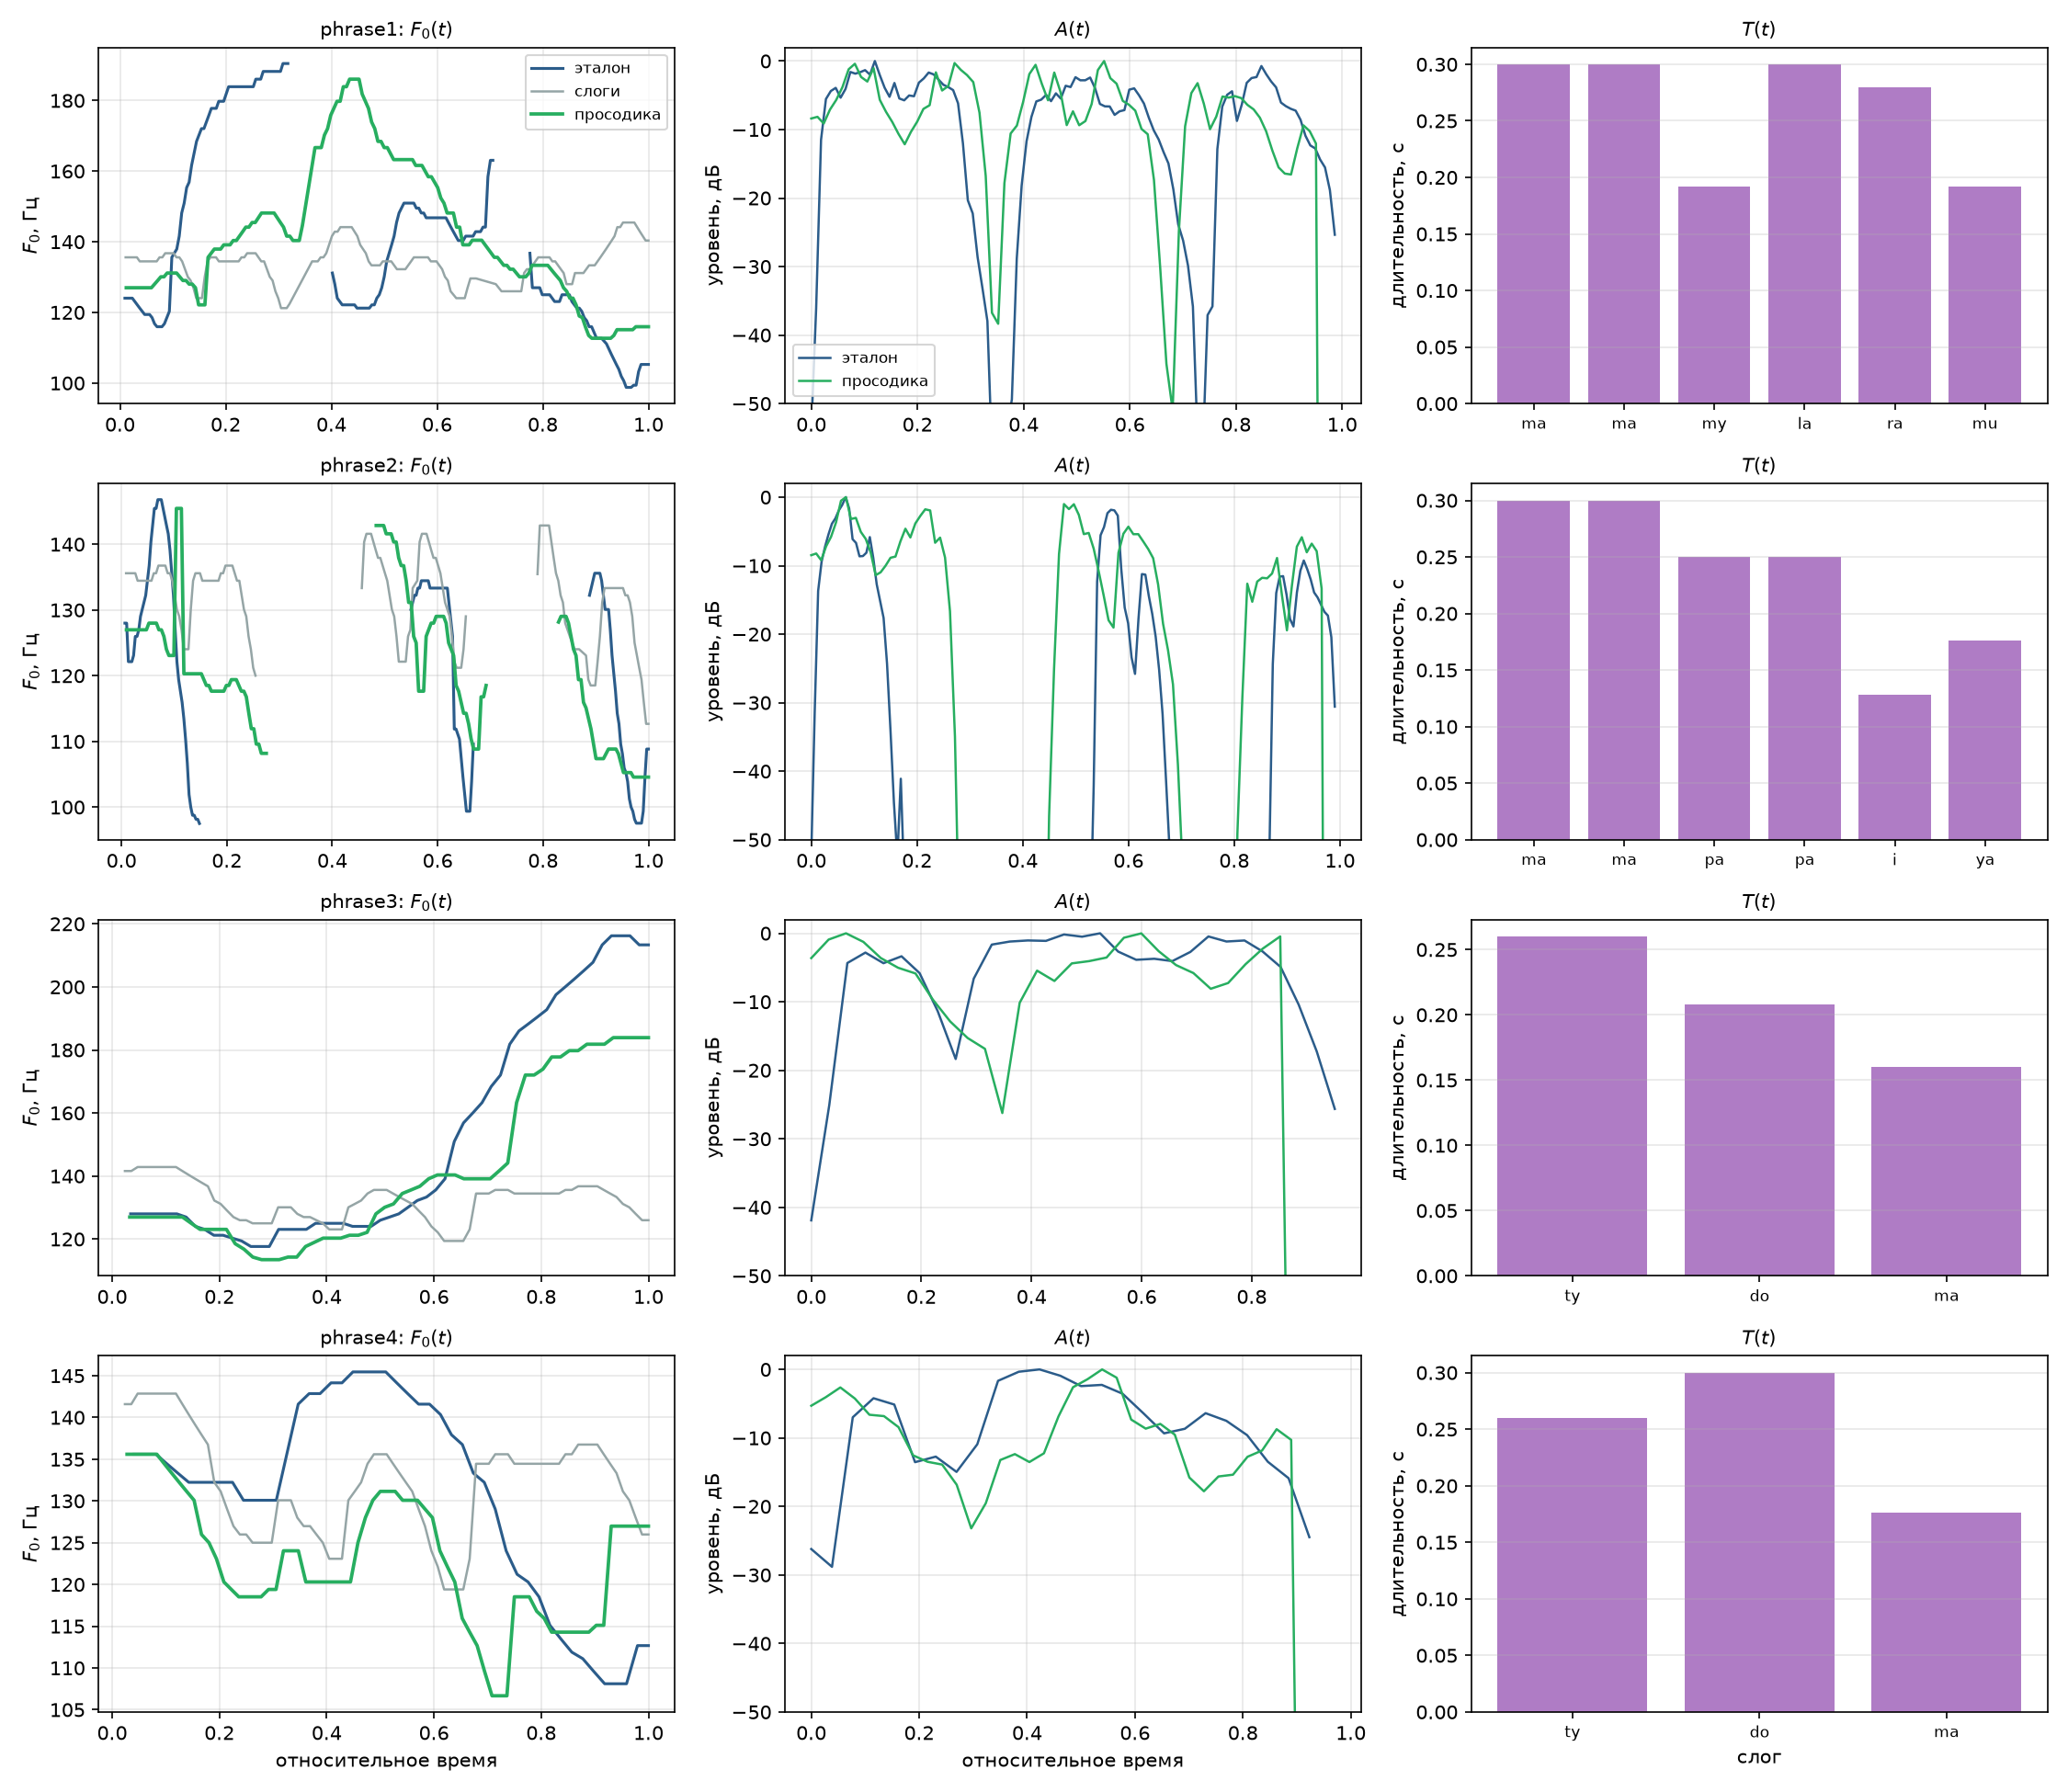
\includegraphics[width=\textwidth]{lab3_prosody_contours.png}
	\caption{Контуры $F_0(t)$, $A(t)$ и $T(t)$ синтезируемых фраз
		(слева направо) в сравнении с эталонами}
	\label{fig:prosody}
\end{figure}

Результаты обработки:
\begin{itemize}
	\item во фразе <<Мама мыла раму.>> тон поднимается к ударному [ы]
	(130 \(\to\) 181~Гц) и понижается к концу (до 115~Гц), повторяя
	нисходящий терминальный контур эталона;
	\item в перечислении <<Мама, папа и я.>> контур в целом понижается с
	127 до 105~Гц, как в эталоне (134 \(\to\) 109~Гц);
	\item вопрос <<Ты дома?>> получил выраженный восходящий контур
	(123 \(\to\) 182~Гц, рост на $+6{,}8$~полутона), тогда как утверждение
	<<Ты дома.>> --- нисходящий (125 \(\to\) 115~Гц, спад на
	$-1{,}5$~полутона); теперь фразы отчётливо различаются на слух.
\end{itemize}
Длительности после обработки приблизились к эталонным (например, вопрос
0,63~с против 0,61~с у эталона и 0,87~с у слоговой компиляции). Таким
образом, управление контурами $F_0(t)$, $A(t)$ и $T(t)$ позволяет получить
из монотонной компиляции интонационно насыщенную речь, близкую к
естественной по мелодике, ритму и громкости.
